\documentclass[12pt]{article}

\title{Activity 2: Bits and Bytes}
\author{Dr. Chris Mayfield}
\date{CS 101, Fall 2016}

%\ProvidesPackage{cspogil}

% fonts
\usepackage[utf8]{inputenc}
\usepackage[T1]{fontenc}
\usepackage{mathpazo}

% spacing
\usepackage[margin=2cm]{geometry}
\renewcommand{\arraystretch}{1.4}
\setlength{\parindent}{0pt}

% orphans and widows
\clubpenalty=10000
\widowpenalty=10000
\pagestyle{empty}

% figures and tables
\usepackage{graphicx}
\usepackage{multicol}
\usepackage{tabularx}
\usepackage{wrapfig}

% fixed-width columns
\usepackage{array}
\newcolumntype{L}[1]{>{\raggedright\let\newline\\\arraybackslash\hspace{0pt}}m{#1}}
\newcolumntype{C}[1]{>{\centering\let\newline\\\arraybackslash\hspace{0pt}}m{#1}}
\newcolumntype{R}[1]{>{\raggedleft\let\newline\\\arraybackslash\hspace{0pt}}m{#1}}

% include paths
\makeatletter
\def\input@path{{Models/}{../../Models/}}
\graphicspath{{Models/}{../../Models/}}
\makeatother

% colors
\usepackage[svgnames,table]{xcolor}
\definecolor{bgcolor}{HTML}{FAFAFA}
\definecolor{comment}{HTML}{007C00}
\definecolor{keyword}{HTML}{0000FF}
\definecolor{strings}{HTML}{B20000}

% table headers
\newcommand{\tr}{\bf\cellcolor{Yellow!10}}

% syntax highlighting
\usepackage{textcomp}
\usepackage{listings}
\lstset{
    basicstyle=\ttfamily\color{black},
    backgroundcolor=\color{bgcolor},
    numberstyle=\scriptsize\color{comment},
    commentstyle=\color{comment},
    keywordstyle=\color{keyword},
    stringstyle=\color{strings},
    columns=fullflexible,
    keepspaces=true,
    showlines=true,
    showstringspaces=false,
    upquote=true
}

% code environments
\newcommand{\java}[1]{\lstinline[language=java]{#1}}%[
\lstnewenvironment{javalst}{\lstset{language=java,backgroundcolor=}}{}
\lstnewenvironment{javabox}{\lstset{language=java,frame=single,numbers=left}\quote}{\endquote}

% PDF properties
\usepackage[pdftex]{hyperref}
\urlstyle{same}
\makeatletter
\hypersetup{
  pdftitle={\@title},
  pdfauthor={\@author},
  pdfsubject={\@date},
  pdfkeywords={},
  bookmarksopen=false,
  colorlinks=true,
  citecolor=black,
  filecolor=black,
  linkcolor=black,
  urlcolor=blue
}
\makeatother

% titles
\makeatletter
\renewcommand{\maketitle}{\begin{center}\LARGE\@title\end{center}}
\makeatother

% boxes [optional height]
\newcommand{\emptybox}[1][10em]{
\vspace{1em}
\begin{tabularx}{\linewidth}{|X|}
\hline\\[#1]\hline
\end{tabularx}}

% models
\newcommand{\model}[1]{\section{#1}\nopagebreak}
\renewcommand{\thesection}{Model~\arabic{section}}

% questions
\newcommand{\quest}[1]{\subsection*{Questions~ (#1)}}
\newcounter{question}
\newcommand{\Q}{\vspace{1em}\refstepcounter{question}\arabic{question}.~ }
\renewcommand{\thequestion}{\#\arabic{question}}

% sub-question lists
\usepackage{enumitem}
\setenumerate[1]{label=\alph*)}
\setlist{itemsep=1em,after=\vspace{1ex}}

% inline answers
\definecolor{answers}{HTML}{C0C0C0}
\newcommand{\ans}[1]{%
\ifdefined\Student
    \leavevmode\phantom{~~\textcolor{answers}{#1}}
\else
    ~~\textcolor{answers}{#1}
\fi}

% longer answers [optional height]
\newsavebox{\ansbox}
\newenvironment{answer}[1][4em]{
\nopagebreak
\begin{lrbox}{\ansbox}
\begin{minipage}[t][#1]{\linewidth}
\color{answers}
}{
\end{minipage}
\end{lrbox}
\ifdefined\Student
    \phantom{\usebox{\ansbox}}%
\else
    \usebox{\ansbox}%
\fi}


\begin{document}

\maketitle

Computer hardware is made up of billions of tiny electronic circuits that use low and high voltages to represent the values 0 and 1.
These binary digits, or ``bits'' for short, are the building blocks of all digital technology.

\model{Logic Gates}

\begin{center}
\textit{Complete the following tables based on the diagrams.}
\end{center}

\begin{minipage}{0.45\textwidth}
\centering
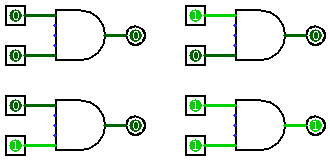
\includegraphics[width=\linewidth]{CSP/logic-and.png}
\par
\vspace{1em}
\begin{tabular}{|C{50pt}|C{50pt}|}
\multicolumn{2}{c}{\sc and} \\
\hline
Inputs & Output \\
\hline
0 ~ 0 &  \\
\hline
0 ~ 1 &  \\
\hline
1 ~ 0 &  \\
\hline
1 ~ 1 &  \\
\hline
\end{tabular}
\end{minipage}
\hfill
\begin{minipage}{0.45\textwidth}
\centering
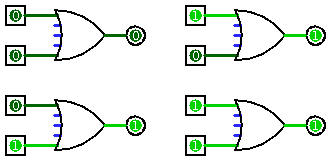
\includegraphics[width=\linewidth]{CSP/logic-or.png}
\par
\vspace{1em}
\begin{tabular}{|C{50pt}|C{50pt}|}
\multicolumn{2}{c}{\sc or} \\
\hline
Inputs & Output \\
\hline
0 ~ 0 &  \\
\hline
0 ~ 1 &  \\
\hline
1 ~ 0 &  \\
\hline
1 ~ 1 &  \\
\hline
\end{tabular}
\end{minipage}

\vspace{2em}

\begin{minipage}[t]{0.45\textwidth}
\centering
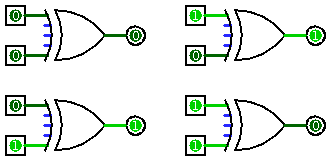
\includegraphics[width=\linewidth]{CSP/logic-xor.png}
\par
\vspace{1em}
\begin{tabular}{|C{50pt}|C{50pt}|}
\multicolumn{2}{c}{\sc xor} \\
\hline
Inputs & Output \\
\hline
0 ~ 0 &  \\
\hline
0 ~ 1 &  \\
\hline
1 ~ 0 &  \\
\hline
1 ~ 1 &  \\
\hline
\end{tabular}
\end{minipage}
\hfill
\begin{minipage}[t]{0.45\textwidth}
\centering

\includegraphics[width=\linewidth]{CSP/logic-not.png}
\par
\vspace{1em}
\begin{tabular}{|C{50pt}|C{50pt}|}
\multicolumn{2}{c}{\sc not} \\
\hline
Input & Output \\
\hline
0 &  \\
\hline
1 &  \\
\hline
\end{tabular}
\end{minipage}


\quest{10 min}


\Q In the circuit diagrams, what does the color (brightness) of the the lines represent?

\begin{answer}
\end{answer}


\Q For each type of gate, describe the circumstances when it will output the value 1.

\begin{description}
\item \textsc{and}:
\item \textsc{or}:
\item \textsc{xor}:
\item \textsc{not}:
\end{description}


\Q As a team, define the following words as they are used in everyday English.

\begin{description}
\item logic:
\item gate:
\end{description}


\Q Based on your definitions, what do you think a ``logic gate'' represents?

\begin{answer}
\end{answer}


\Q In the example circuit below, what are the values of $A$, $B$, $C$, $D$, and $E$?

\vspace{1em}
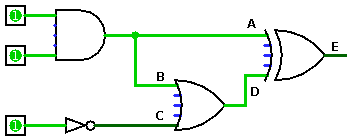
\includegraphics[width=0.45\textwidth]{CSP/logic-example.png}
\vspace{1em}


\Q How would $A$, $B$, $C$, $D$, and/or $E$ change if the top input were zero?

\begin{answer}
\end{answer}

% Based on Model 1 from "Activity 5 - Binary" by Helen Hu
% which in turn uses "Count the Dots" from csunplugged.org

\model{Binary Numbers}

Each team has four cards that are ordered from the card with the most dots (8) to the card with the least dots (1). The cards represent four binary digits, or in other words, a 4-bit number.

\newcommand{\bin}[4]{#1\hspace{64pt}#2\hspace{64pt}#3\hspace{64pt}#4}

\begin{center}
\begin{tabular}{|c|C{1in}|}
\hline
Binary & Decimal \\
\hline
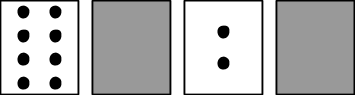
\includegraphics[height=1in]{CSP/binary1.png} & \\
\bin{1}{0}{1}{0} & \\
\hline
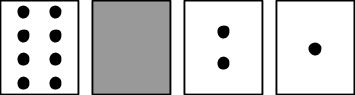
\includegraphics[height=1in]{CSP/binary2.png} & \\
\bin{1}{0}{1}{1} & \\
\hline
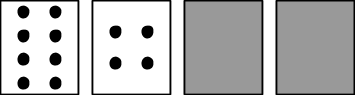
\includegraphics[height=1in]{CSP/binary3.png} & \\
\bin{1}{1}{0}{0} & \\
\hline
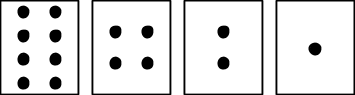
\includegraphics[height=1in]{CSP/binary4.png} & \\
\bin{1}{1}{1}{1} & \\
\hline
\end{tabular}
\end{center}


\quest{15 min}


\Q \label{fourbit} In the table above, write the decimal value for each row by counting the number of dots.
\begin{enumerate}
\item What is the largest decimal number that can be represented by four bits?
\item What is the smallest decimal number that can be represented by four bits?
\item How many possible decimal numbers can be represented by four bits?
\end{enumerate}


\Q Examine the binary notation below the cards. Explain in a full sentence what a 0 means about the card's dots and what a 1 means.

\begin{answer}
\end{answer}


\Q \label{binhex} Complete the following table by writing the binary representation of the decimal numbers 0 to 15 using four bits. (And check your answers for \ref{fourbit}.)

\begin{center}
\begin{tabular}{|C{1in}|C{1in}|C{1in}|}
\hline
Decimal & Binary & Hex \\
\hline
0  &  & 0 \\
\hline
1  &  & 1 \\
\hline
2  &  & 2 \\
\hline
3  &  & 3 \\
\hline
4  &  & 4 \\
\hline
5  &  & 5 \\
\hline
6  &  & 6 \\
\hline
7  &  & 7 \\
\hline
8  &  & 8 \\
\hline
9  &  & 9 \\
\hline
10 &  & A \\
\hline
11 &  & B \\
\hline
12 &  & C \\
\hline
13 &  & D \\
\hline
14 &  & E \\
\hline
15 &  & F \\
\hline
\end{tabular}
\end{center}


\Q \emph{Hexadecimal} is shorthand for binary. For example, 0xD5 in hex is 1101 0101.

\begin{enumerate}
\item What is 0x2E in binary?
\item What is 0x74 in binary?
\item What is 0xB00 in binary?
\item What is 0xFAD in binary?
\end{enumerate}


\Q Based on the table in \ref{binhex}, explain why binary is sometimes referred to as base-2, decimal as base-10, and hexadecimal as base-16.

\begin{answer}
\end{answer}


\Q Explain the humor: ``There are only 10 types of people in the world: those who understand binary, and those who don't.''

\begin{answer}
\end{answer}


\Q Typically computers group 8 bits together at a time (8 bits are also called 1 \emph{byte}). Fill in the number of dots for the four new cards:

\begin{center}
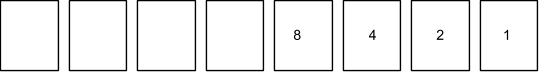
\includegraphics[width=\textwidth]{CSP/binary5.png}
\end{center}


\Q What is the largest number that can be represented by:
\begin{enumerate}
\item five bits?
\item six bits?
\item seven bits?
\item eight bits?
\item $n$ bits?
\end{enumerate}


\Q Most computers built since the year 2000 have 64-bit processors. Before then, 32-bit processors were the norm. What is the advantage of having more bits?

\begin{answer}
\end{answer}


\Q In terms of logic gates and digital circuits, what is the disadvantage of having more bits?

\begin{answer}
\end{answer}


\end{document}
